\documentclass[aspectratio=169]{beamer}
\usetheme{Madrid}
\usecolortheme{default}
\usepackage[utf8]{inputenc}
\usepackage[T5]{fontenc}
\usepackage{graphicx}
\usepackage{hyperref}
\usepackage{booktabs}
\usepackage{amsmath}

% Thêm package listings để hiển thị code
\usepackage{listings}
\usepackage{xcolor}

\definecolor{codegreen}{rgb}{0,0.6,0}
\definecolor{codegray}{rgb}{0.5,0.5,0.5}
\definecolor{codepurple}{rgb}{0.58,0,0.82}
\definecolor{backcolour}{rgb}{0.95,0.95,0.92}

\lstdefinestyle{mystyle}{
    backgroundcolor=\color{backcolour},   
    commentstyle=\color{codegreen},
    keywordstyle=\color{magenta},
    numberstyle=\tiny\color{codegray},
    stringstyle=\color{codepurple},
    basicstyle=\ttfamily\footnotesize,
    breakatwhitespace=false,         
    breaklines=true,                 
    captionpos=b,                    
    keepspaces=true,                 
    numbers=left,                    
    numbersep=5pt,                  
    showspaces=false,                
    showstringspaces=false,
    showtabs=false,                  
    tabsize=2
}
\lstset{style=mystyle}

\setbeamertemplate{caption}[numbered]
\renewcommand{\figurename}{Hình}
\renewcommand{\thefigure}{4.\arabic{figure}}

\title[Chương 4: Phân loại \& Hồi quy]{Học Sâu (Deep Learning) \\ \vspace{0.5cm} \Large Chương 4: Bắt đầu với Mạng Nơ-ron (Phân loại và Hồi quy)}
\author{Đại học Đông Á}
\date{\today}

\begin{document}

\begin{frame}
    \titlepage
\end{frame}

\begin{frame}{Nội dung chương}
    \tableofcontents
\end{frame}

\section{1. Các thuật ngữ cốt lõi (Glossary)}

\begin{frame}{Khái niệm Cơ bản}
    Trong phân loại và hồi quy, các kỹ sư Học máy sử dụng thuật ngữ rất nghiêm ngặt:
    \begin{itemize}
        \item \textbf{Sample (Mẫu / Đầu vào):} Một điểm dữ liệu đi vào mô hình. Ví dụ: Một bức ảnh, một đoạn văn bản.
        \item \textbf{Target (Mục tiêu / Sự thật):} Kết quả kỳ vọng. Mô hình lý tưởng sẽ dự đoán ra kết quả này theo một tập dữ liệu chuẩn.
        \item \textbf{Prediction (Dự đoán / Đầu ra):} Giá trị đầu ra thực tế từ mô hình của bạn.
        \item \textbf{Loss value (Giá trị mất mát):} Khoảng cách đo lường sự chênh lệch giữa Prediction (Dự đoán) và Target (Mục tiêu).
    \end{itemize}
\end{frame}

\begin{frame}{Thuật ngữ về Nhãn (Labels \& Classes)}
    \begin{itemize}
        \item \textbf{Classes (Lớp):} Tập hợp các danh mục khả dĩ trong một bài toán phân loại. (Ví dụ: Chó, Mèo, Chim).
        \item \textbf{Label (Nhãn):} Một phiên bản cụ thể của Class được gán cho một Sample. Ví dụ: Ảnh \#1234 có nhãn là "Chó".
        \item \textbf{Ground-truth (Sự thật gốc):} Toàn bộ các targets của tập dữ liệu, thường được con người thu thập và gán nhãn thủ công.
        \item \textbf{Batch (Mini-batch - Lô):} Một tập hợp nhỏ các samples (thường 8-128) được mô hình xử lý cùng lúc để tính gradient. Kích thước batch thường là lũy thừa của 2 để tối ưu bộ nhớ GPU.
    \end{itemize}
\end{frame}

\begin{frame}{Phân loại các bài toán Học máy cơ bản}
    Có 3 bài toán phổ biến nhất trên dữ liệu dạng vector (bảng):
    \begin{enumerate}
        \item \textbf{Phân loại Nhị phân (Binary Classification):} Phân loại đầu vào thành 2 nhóm độc quyền (Ví dụ: Chó hoặc Mèo, Positive hoặc Negative).
        \item \textbf{Phân loại Đa lớp (Multiclass Classification):} Phân loại đầu vào thành nhiều hơn 2 nhóm. Nếu mỗi mẫu chỉ thuộc 1 danh mục duy nhất, ta gọi là bài toán Single-label Multiclass. (Ví dụ: Nhận dạng chữ số 0-9).
        \item \textbf{Hồi quy Vô hướng (Scalar Regression):} Dự đoán một giá trị mục tiêu liên tục (vô hướng). (Ví dụ: Dự đoán giá nhà, nhiệt độ).
    \end{enumerate}
\end{frame}

\begin{frame}[fragile]{Chuẩn bị dữ liệu (Data Preprocessing)}
    Mạng nơ-ron không nhận dữ liệu thô (chuỗi văn bản có độ dài khác nhau). Chúng ta phải biến danh sách từ vựng thành tensor:
    \begin{itemize}
        \item \textbf{Mã hóa đa điểm (Multi-hot Encoding):} Biến danh sách thành các vector 0 và 1 (chỉ số xuất hiện). Ví dụ: \texttt{[8, 5]} thành vector toàn 0, ngoại trừ chỉ số 5 và 8 là 1.
    \end{itemize}
\begin{lstlisting}[language=Python]
import numpy as np
def multi_hot_encode(sequences, num_classes):
    results = np.zeros((len(sequences), num_classes))
    for i, sequence in enumerate(sequences):
        results[i, sequence] = 1.0  # Dat 1 tai cac vi tri tu xuat hien
    return results
\end{lstlisting}
\end{frame}

\section{2. Phân loại Nhị phân (IMDb Dataset)}

\begin{frame}{Bài toán Đánh giá Cảm xúc (IMDb Dataset)}
    \begin{itemize}
        \item \textbf{Mục tiêu:} Đánh giá xem một bài bình luận phim (movie review) là Tích cực (Positive - 1) hay Tiêu cực (Negative - 0).
        \item \textbf{Dữ liệu:} 50.000 bài đánh giá từ Internet Movie Database, chia đều 25.000 train và 25.000 test. Cân bằng 50\% Positive - 50\% Negative.
        \item \textbf{Tiền xử lý dữ liệu:} Từ ngữ được mã hóa thành các số nguyên (integer index). Ta sẽ dùng \texttt{num\_words=10000} để chỉ giữ 10.000 từ xuất hiện phổ biến nhất, loại bỏ các từ quá hiếm.
    \end{itemize}
\end{frame}

\begin{frame}[fragile]{Tải và Khám phá tập dữ liệu IMDb}
\begin{lstlisting}[language=Python]
from keras.datasets import imdb

# Tai 10000 tu pho bien nhat
(train_data, train_labels), (test_data, test_labels) = imdb.load_data(num_words=10000)

# Kiem tra dong du lieu dau tien
print(train_data[0]) 
# [1, 14, 22, 16, 43, 530, 973, 1622, ... 178, 32]
print(train_labels[0]) 
# 1 (Tich cuc)
\end{lstlisting}
    Mỗi bài đánh giá đã được Keras mã hóa sẵn thành chuỗi số nguyên. Ta không phải xử lý văn bản thô (raw text) từ đầu.
\end{frame}

\begin{frame}[fragile]{Chuẩn bị Dữ liệu (Vector hóa)}
    Như đã thảo luận, ta dùng Multi-hot Encoding để biến chuỗi có độ dài thay đổi thành Vector 10000 chiều:
\begin{lstlisting}[language=Python]
import numpy as np

# Vector hoa input (su dung ham multi_hot_encode)
x_train = multi_hot_encode(train_data, num_classes=10000)
x_test = multi_hot_encode(test_data, num_classes=10000)

# Label da la so nguyen 0 hoac 1, ta chi can chuyen sang float32
y_train = train_labels.astype("float32")
y_test = test_labels.astype("float32")
\end{lstlisting}
\end{frame}

\begin{frame}{Kiến trúc Mạng Nơ-ron 3 Lớp}
    \begin{columns}
        \column{0.5\textwidth}
        \begin{itemize}
            \item Mạng có 2 lớp ẩn (Hidden Layers), mỗi lớp có 16 nơ-ron (units).
            \item Lớp đầu ra (Output Layer) có 1 nơ-ron để đưa ra dự đoán vô hướng (xác suất).
            \item Ý nghĩa: Lớp thứ nhất trích xuất đặc trưng cơ bản. Lớp thứ hai phân tích quan hệ phức tạp. Lớp cuối tổng hợp kết quả.
        \end{itemize}
        
        \column{0.5\textwidth}
        \begin{figure}
            \centering
            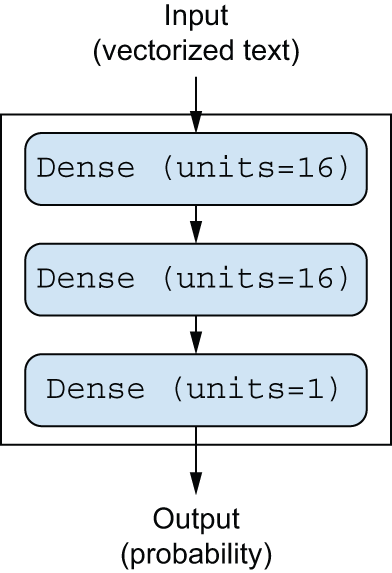
\includegraphics[width=\textwidth,height=0.7\textheight,keepaspectratio]{../../images/ch04/3_layer_network.cf1b1cd7.png}
            \caption{Cấu trúc mạng 3 lớp cho phân loại IMDb}
        \end{figure}
    \end{columns}
\end{frame}

\begin{frame}[fragile]{Định nghĩa Mô hình trong Keras}
    Ta sử dụng \texttt{keras.Sequential} để chồng các lớp liên tiếp nhau. Lớp Dense 16 units cần một hàm kích hoạt phi tuyến tính.
\begin{lstlisting}[language=Python]
import keras
from keras import layers

model = keras.Sequential([
    layers.Dense(16, activation="relu"),
    layers.Dense(16, activation="relu"),
    layers.Dense(1, activation="sigmoid")
])
\end{lstlisting}
\end{frame}

\begin{frame}{Hàm kích hoạt (Activation): ReLU}
    \begin{columns}
        \column{0.5\textwidth}
        \begin{equation}
            f(x) = \max(0, x)
        \end{equation}
        \begin{itemize}
            \item \textbf{ReLU (Rectified Linear Unit):} Loại bỏ giá trị âm (trả về 0), giữ nguyên giá trị dương.
            \item Nếu không có hàm kích hoạt phi tuyến, mạng nhiều lớp cũng chỉ tương đương 1 lớp tuyến tính, không thể giải quyết bài toán phức tạp.
        \end{itemize}
        
        \column{0.5\textwidth}
        \begin{figure}
            \centering
            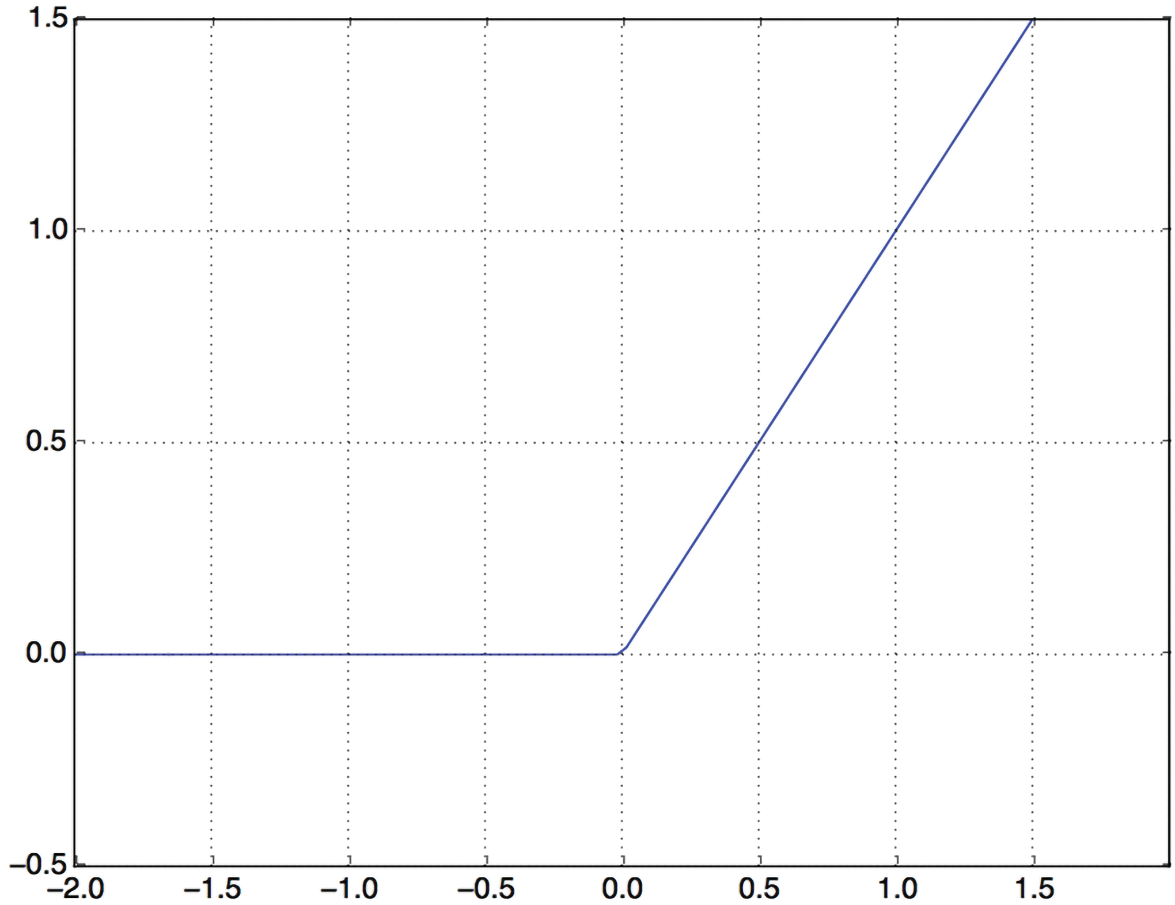
\includegraphics[width=\textwidth,height=0.7\textheight,keepaspectratio]{../../images/ch04/The-rectified-linear-unit-function.351095bf.png}
            \caption{Đồ thị của hàm ReLU}
        \end{figure}
    \end{columns}
\end{frame}

\begin{frame}{Lớp Output: Hàm Sigmoid}
    \begin{columns}
        \column{0.5\textwidth}
        \begin{equation}
            f(x) = \frac{1}{1 + e^{-x}}
        \end{equation}
        \begin{itemize}
            \item Đầu ra của mạng có thể là số bất kỳ $(-\infty, +\infty)$.
            \item \textbf{Sigmoid:} Ép bất kỳ giá trị nào về miền xác suất $[0, 1]$.
            \item Ví dụ: Kết quả $0.9 \rightarrow$ Mô hình có $90\%$ tự tin đây là bình luận Tích cực.
        \end{itemize}
        
        \column{0.5\textwidth}
        \begin{figure}
            \centering
            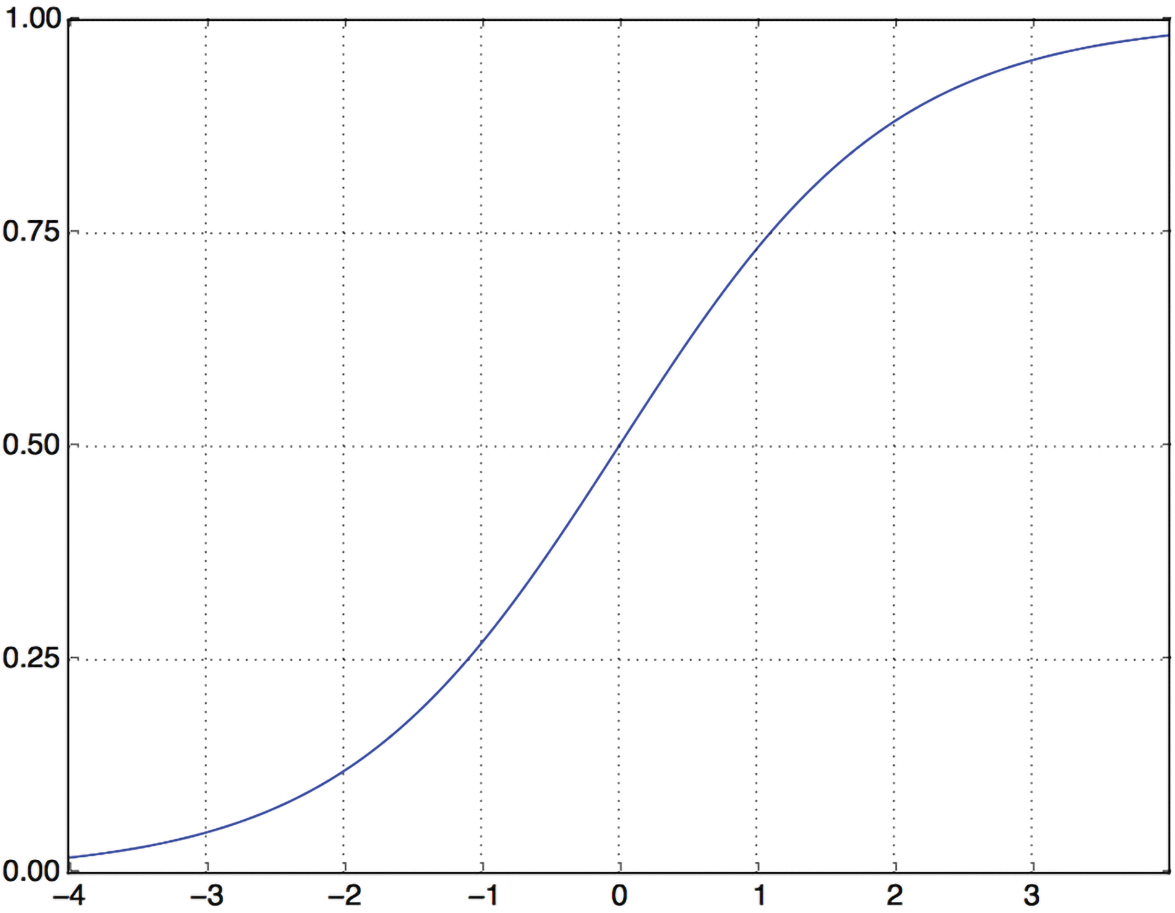
\includegraphics[width=\textwidth,height=0.7\textheight,keepaspectratio]{../../images/ch04/The-sigmoid-function.eac1368d.png}
            \caption{Đồ thị của hàm Sigmoid}
        \end{figure}
    \end{columns}
\end{frame}

\begin{frame}[fragile]{Biên dịch (Compile) và Xác thực (Validation)}
    Bài toán phân loại nhị phân sử dụng độ đo Loss là \texttt{binary\_crossentropy}. Thuật toán tối ưu phổ quát là \texttt{adam}.
\begin{lstlisting}[language=Python]
model.compile(optimizer="adam",
              loss="binary_crossentropy",
              metrics=["accuracy"])

# Huan luyen va theo doi tren tap Validation 20%
history = model.fit(x_train,
                    y_train,
                    epochs=20,
                    batch_size=512,
                    validation_split=0.2)
\end{lstlisting}
\end{frame}

\begin{frame}{Đánh giá Huấn luyện: Biểu đồ Loss}
    \begin{columns}
        \column{0.5\textwidth}
        \begin{itemize}
            \item Đường chấm bi (Training Loss) liên tục giảm $\rightarrow$ Mô hình đang học rất tốt dữ liệu đào tạo.
            \item Đường liền (Validation Loss) giảm xuống mức tối thiểu tại epoch 4, sau đó đột ngột tăng lại.
            \item \textbf{Overfitting (Quá khớp):} Mô hình học thuộc lòng dữ liệu train nhưng không có khả năng tổng quát hóa dữ liệu chưa từng thấy.
        \end{itemize}
        
        \column{0.5\textwidth}
        \begin{figure}
            \centering
            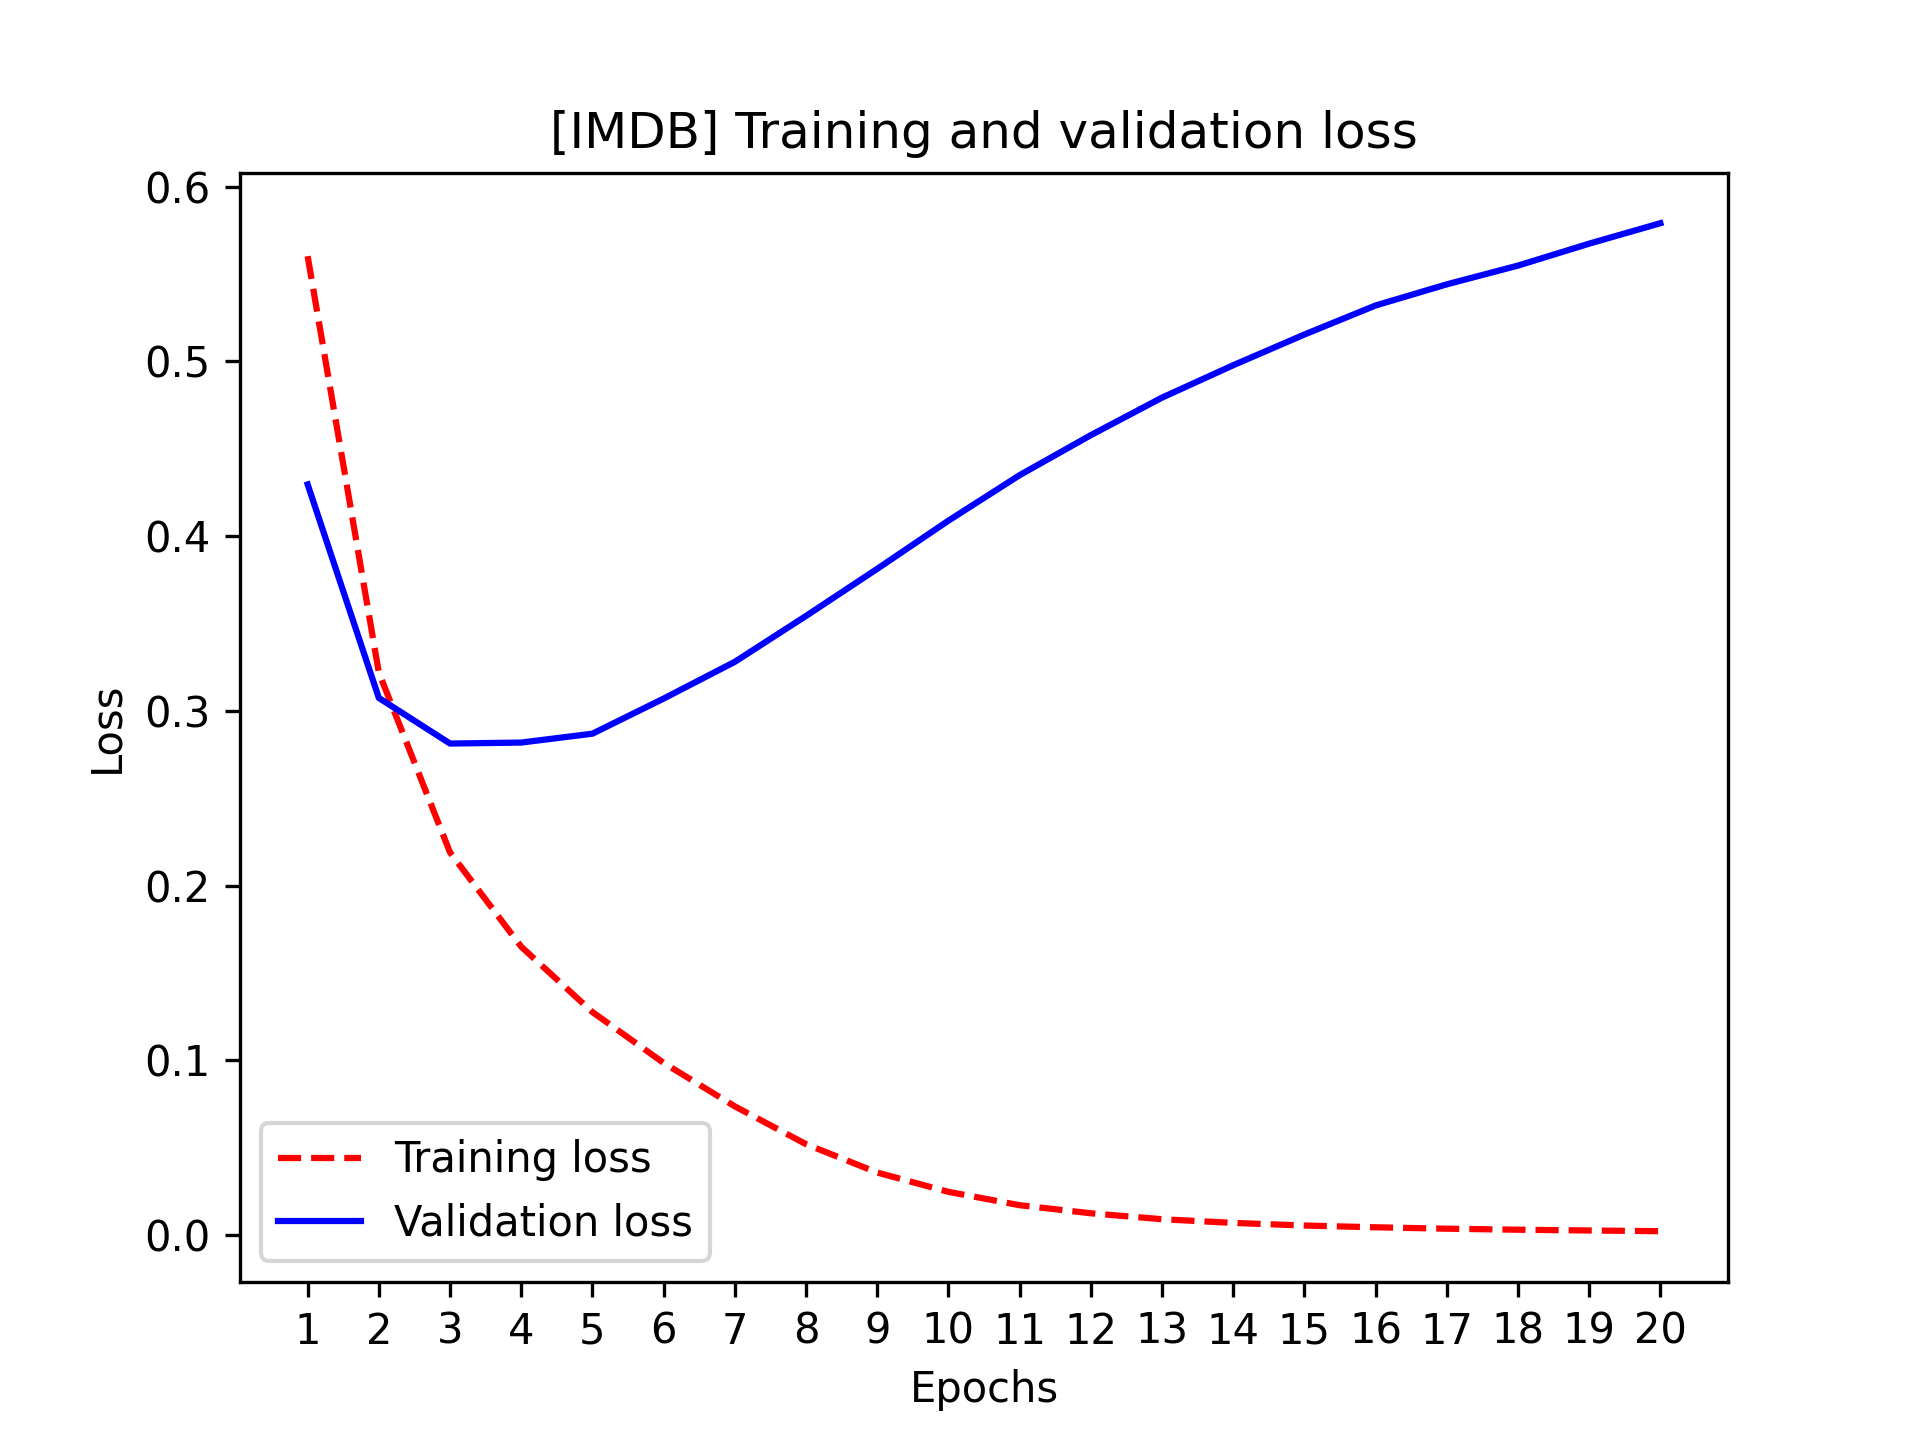
\includegraphics[width=\textwidth,height=0.7\textheight,keepaspectratio]{../../images/ch04/imdb_loss_plot.801b28d0.png}
            \caption{Sự thay đổi Loss qua các Epochs}
        \end{figure}
    \end{columns}
\end{frame}

\begin{frame}{Đánh giá Huấn luyện: Biểu đồ Accuracy}
    \begin{columns}
        \column{0.5\textwidth}
        \begin{itemize}
            \item Training Accuracy (chấm bi) tiến sát 100\% (1.0).
            \item Validation Accuracy (đường liền) đạt đỉnh khoảng 88\% tại epoch thứ 4, sau đó giảm dần.
            \item \textbf{Giải pháp:} Ta nên huấn luyện lại một mô hình mới, cài đặt \texttt{epochs=4} (Early Stopping) để lấy kết quả tốt nhất.
        \end{itemize}
        
        \column{0.5\textwidth}
        \begin{figure}
            \centering
            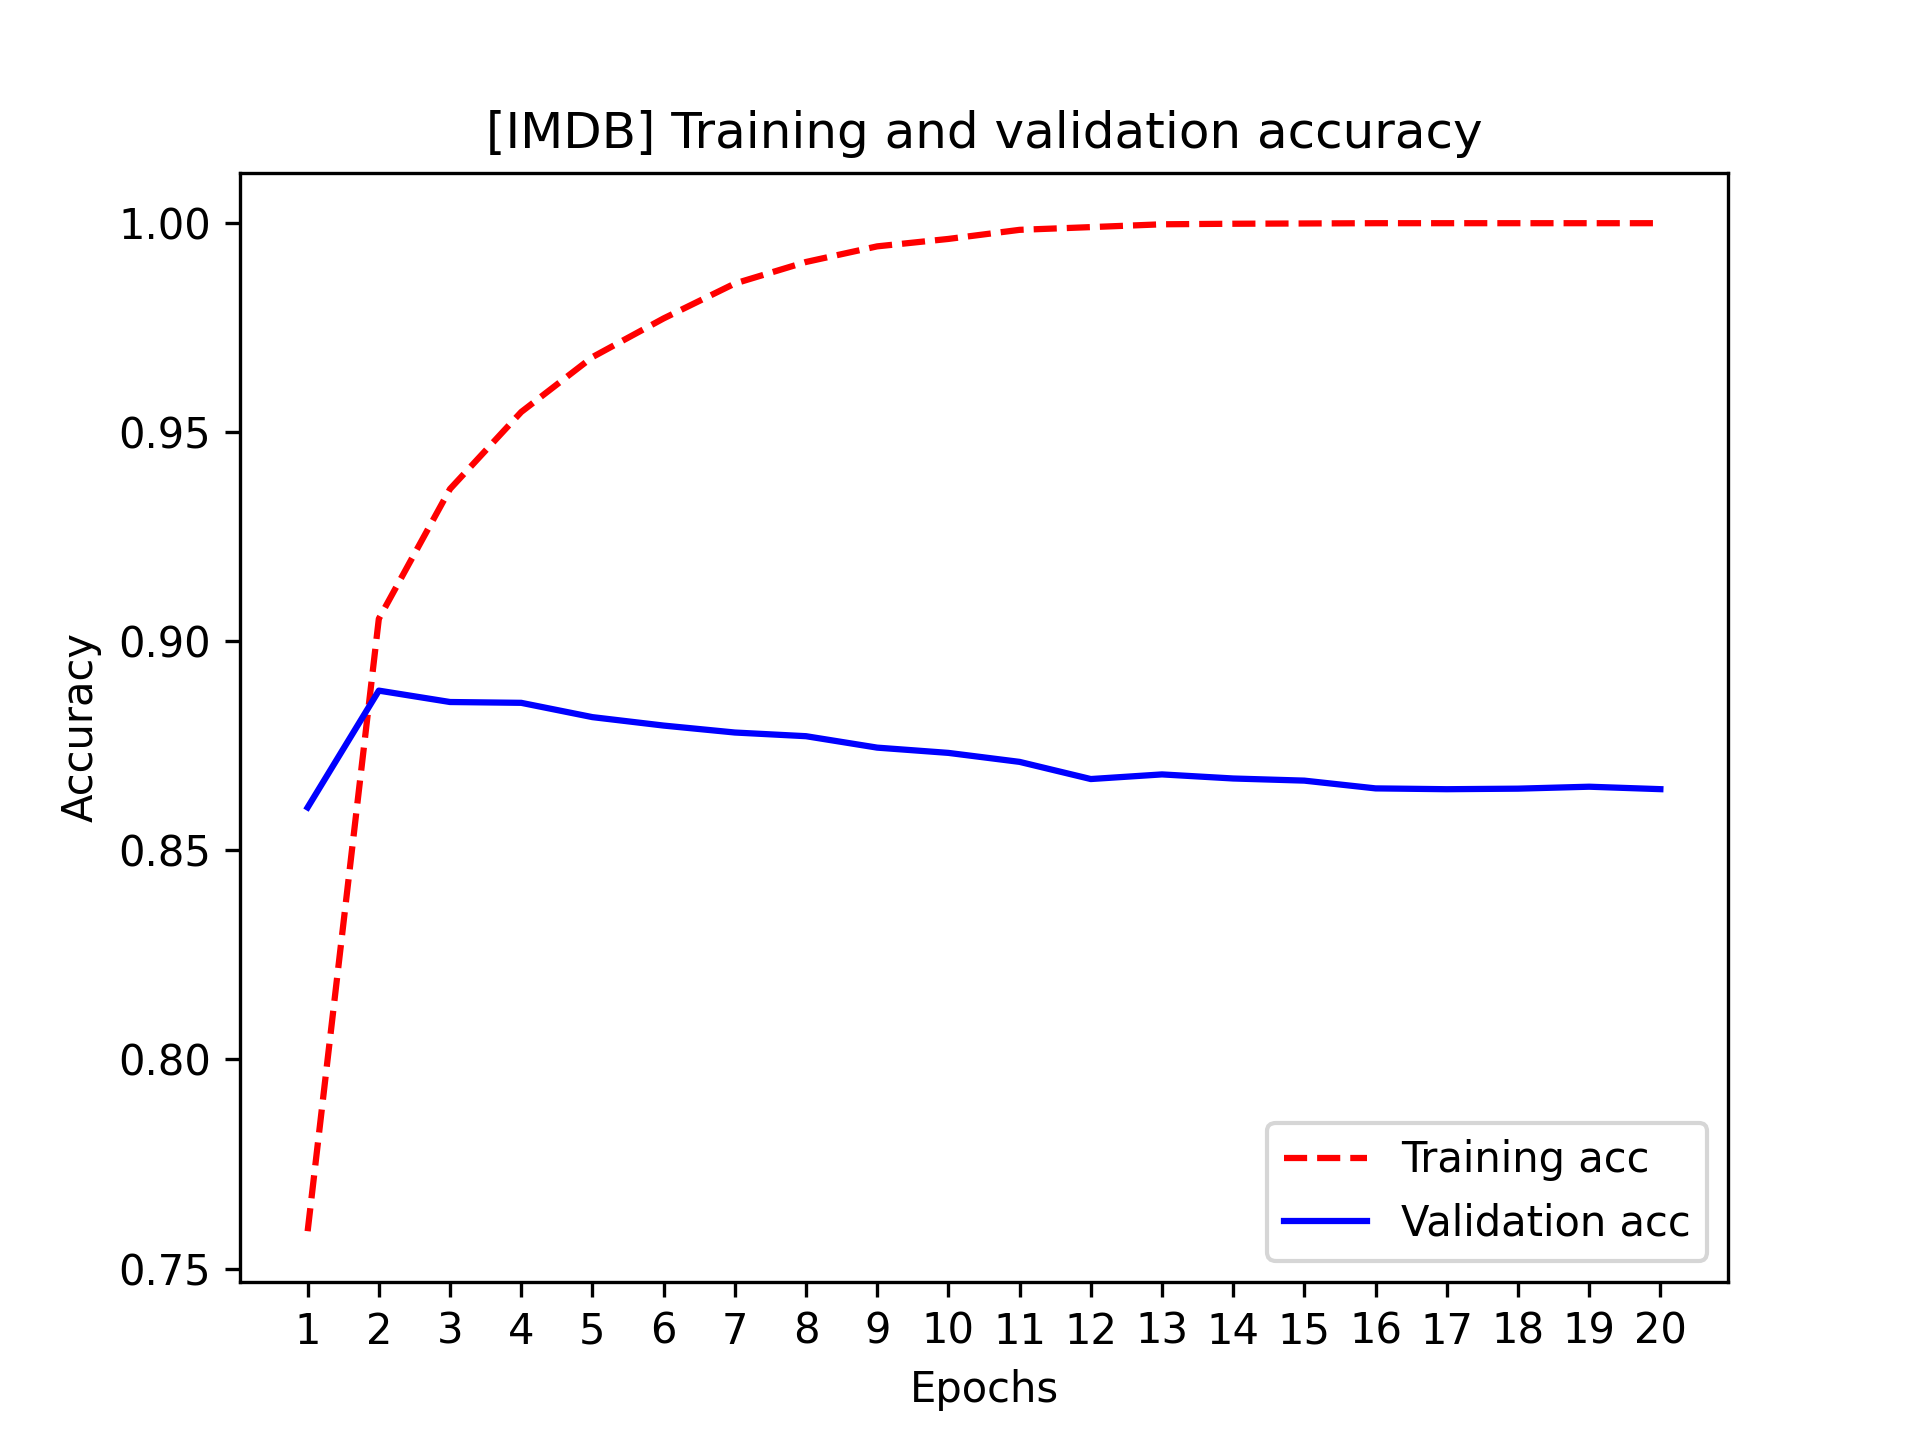
\includegraphics[width=\textwidth,height=0.7\textheight,keepaspectratio]{../../images/ch04/imdb_accuracy_plot.bf0cb7ef.png}
            \caption{Sự biến thiên của Accuracy}
        \end{figure}
    \end{columns}
\end{frame}

\begin{frame}[fragile]{Dự đoán dữ liệu mới (Predictions)}
    Sau khi có mô hình tốt nhất (train 4 epochs), ta có thể sử dụng hàm \texttt{predict()} để đánh giá dữ liệu mới ngoài thực tế.
\begin{lstlisting}[language=Python]
predictions = model.predict(x_test)
print(predictions)
# array([[ 0.98006207], 
#        [ 0.99758697], 
#        ..., 
#        [ 0.02885115], 
#        [ 0.65371346]], dtype=float32)
\end{lstlisting}
    \textbf{Nhận xét:} Mô hình cực kỳ tự tin với một số mẫu (0.99 - rất Tích cực, hoặc 0.02 - rất Tiêu cực). Nhưng với 0.65, nó còn lưỡng lự.
\end{frame}


\section{3. Phân loại Đa lớp (Reuters Dataset)}

\begin{frame}{Bài toán Reuters (Multiclass Classification)}
    \begin{itemize}
        \item \textbf{Mục tiêu:} Phân loại các bản tin tức (Newswires) của hãng thông tấn Reuters vào 46 chủ đề khác nhau.
        \item \textbf{Đặc trưng bài toán:} Đây là bài toán \textbf{Single-label, Multiclass} (Mỗi bài báo chỉ thuộc duy nhất 1 chủ đề, nhưng có tới 46 chủ đề để lựa chọn).
        \item Dữ liệu có 8982 mẫu huấn luyện và 2246 mẫu kiểm tra.
        \item \textbf{Chuẩn bị:} Dữ liệu đầu vào text cũng được dùng Multi-hot Encoding tương tự như IMDb.
    \end{itemize}
\end{frame}

\begin{frame}[fragile]{Mã hóa Nhãn (One-Hot Encoding Labels)}
    Ở IMDb có 2 nhãn (0, 1) nên ta dùng số nguyên. Ở Reuters có 46 chủ đề, ta phải biến đổi mảng nhãn thành dạng Vector qua \textbf{One-hot encoding} (Mã hóa phân loại).
\begin{lstlisting}[language=Python]
from keras.utils import to_categorical

# Chuyen [3, 10, 45, ...] thanh ma tran 46 cot (0 va 1)
y_train = to_categorical(train_labels)
y_test = to_categorical(test_labels)

# y_train[0] co nhan '3' -> se la vector gom 45 so 0 va so 1 tai index 3.
\end{lstlisting}
\end{frame}

\begin{frame}[fragile]{Kiến trúc Mô hình Đa lớp}
    \begin{itemize}
        \item \textbf{Thắt cổ chai thông tin:} Lớp Dense 16 units là quá nhỏ để truyền tải 46 chủ đề. Thông tin sẽ bị mất mát vĩnh viễn. Ta phải tăng lên 64 units.
        \item \textbf{Lớp đầu ra:} Có 46 units (đại diện 46 chủ đề) kết hợp hàm kích hoạt \textbf{Softmax}.
    \end{itemize}
\begin{lstlisting}[language=Python]
model = keras.Sequential([
    layers.Dense(64, activation="relu"),
    layers.Dense(64, activation="relu"),
    layers.Dense(46, activation="softmax")
])
\end{lstlisting}
\end{frame}

\begin{frame}[fragile]{Biên dịch Mô hình Đa lớp}
    \textbf{Softmax} sẽ xuất ra một phân phối xác suất gồm 46 chiều, tổng xác suất luôn bằng 1. Ta cần dùng loss \texttt{categorical\_crossentropy} để đo khoảng cách giữa 2 phân phối xác suất.
\begin{lstlisting}[language=Python]
model.compile(optimizer="adam",
              loss="categorical_crossentropy",
              metrics=["accuracy"])

history = model.fit(x_train,
                    y_train,
                    epochs=20,
                    batch_size=512,
                    validation_split=0.2)
\end{lstlisting}
\end{frame}

\begin{frame}{Hàm mất mát \& Biểu đồ Loss (Reuters)}
    \begin{columns}
        \column{0.5\textwidth}
        \begin{itemize}
            \item \textbf{Categorical Crossentropy}: Chuyên dụng đo lường khoảng cách giữa hai phân phối xác suất đa chiều.
            \item Hiện tượng \textbf{Overfitting} (Quá khớp) xảy ra ở hầu như mọi bài toán Học sâu. Tại Reuters, Loss trên tập validation bắt đầu tăng mạnh sau epoch thứ 9.
        \end{itemize}
        
        \column{0.5\textwidth}
        \begin{figure}
            \centering
            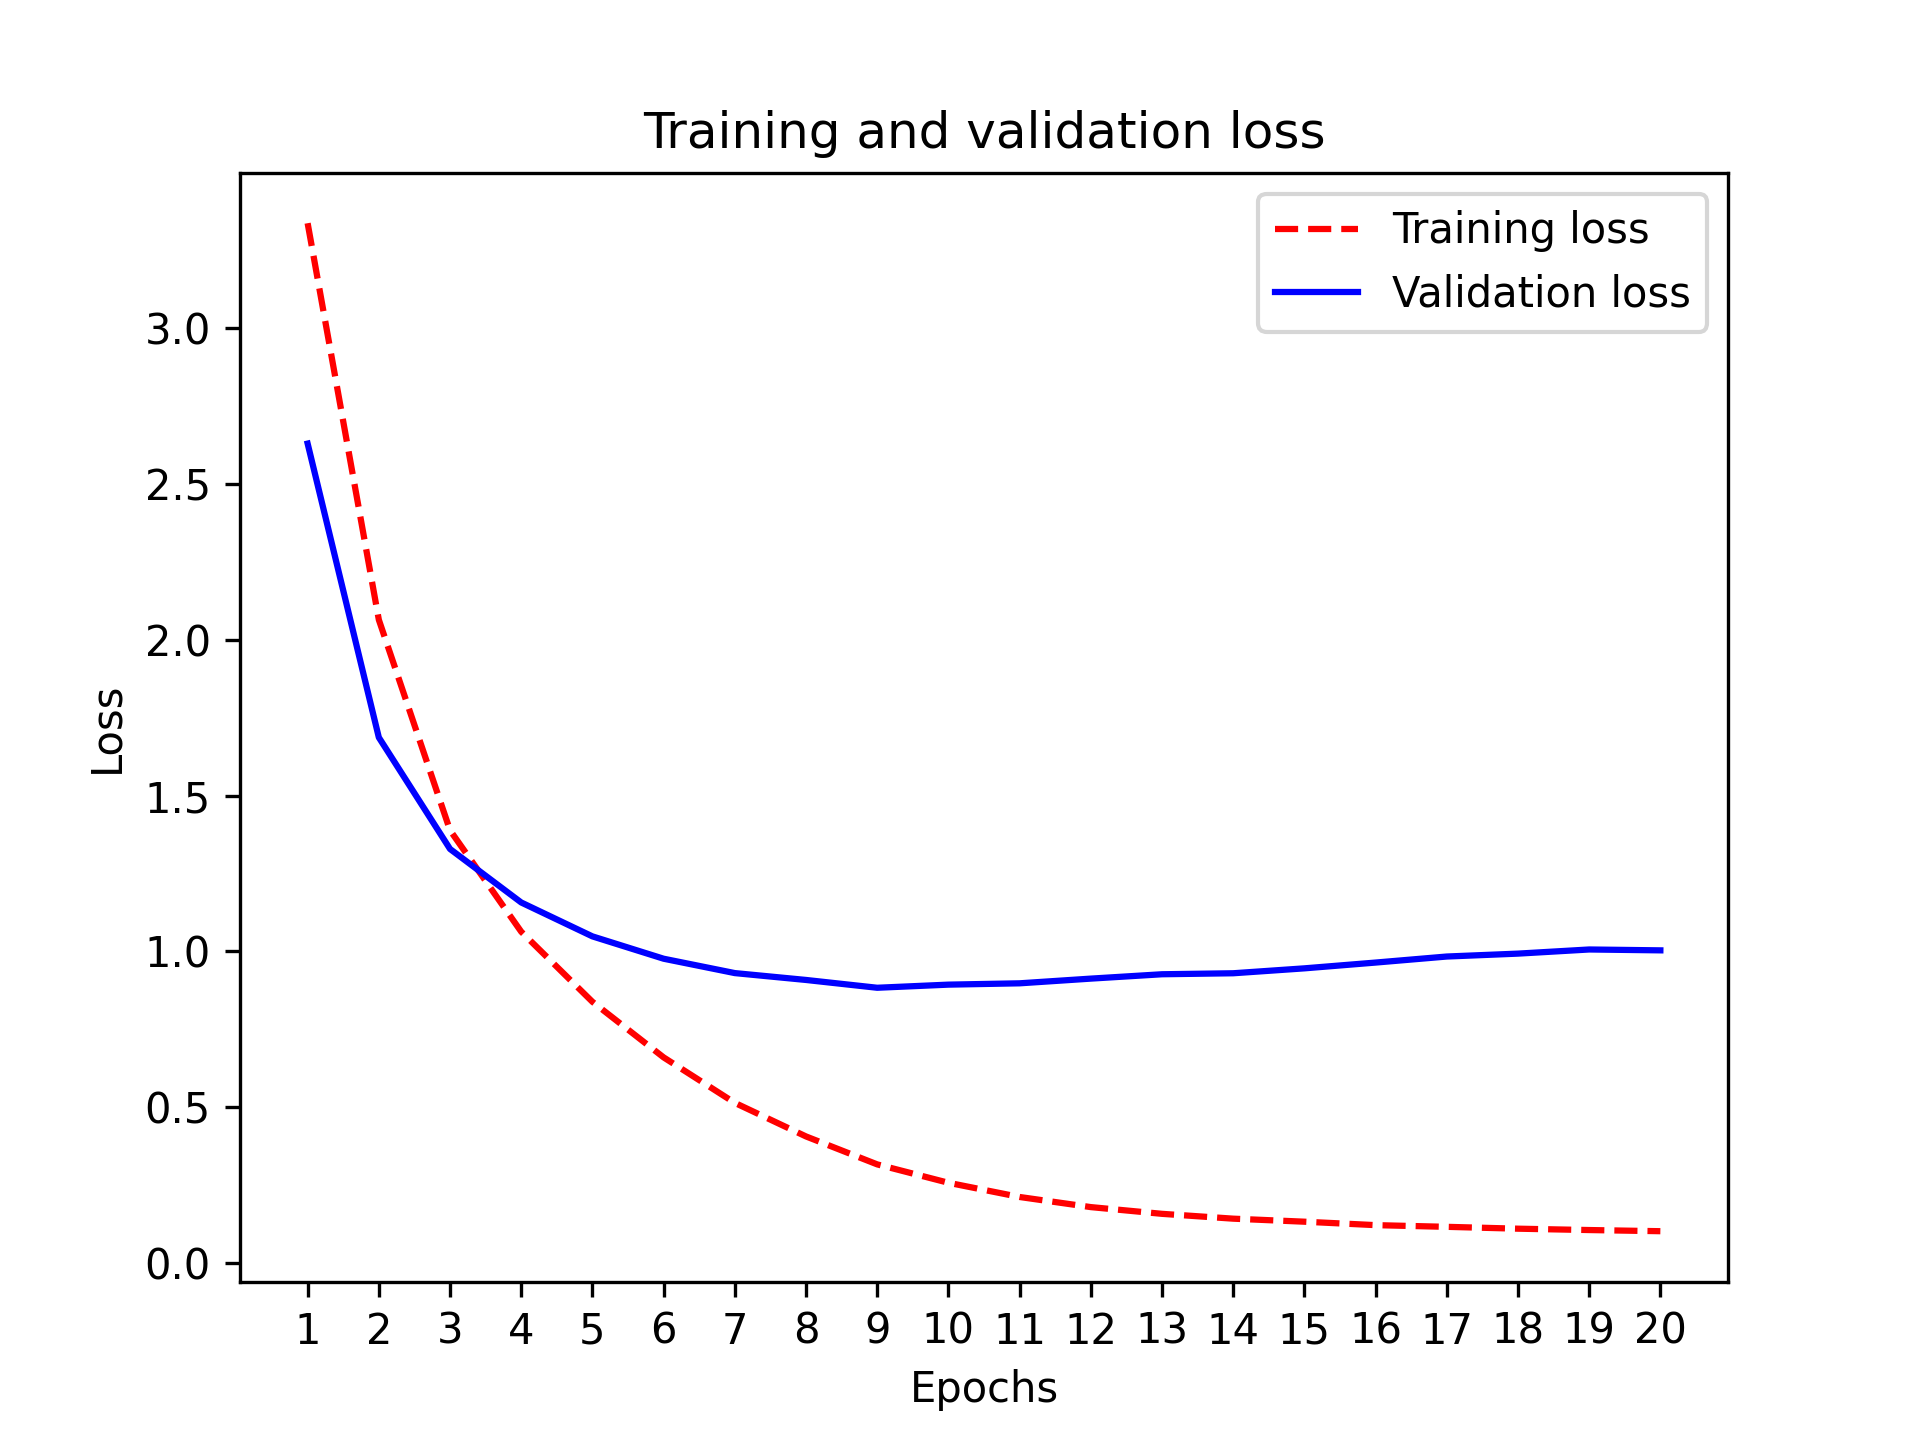
\includegraphics[width=\textwidth,height=0.7\textheight,keepaspectratio]{../../images/ch04/reuters_loss_plot.6e487e1a.png}
            \caption{Training và Validation Loss (Reuters)}
        \end{figure}
    \end{columns}
\end{frame}

\begin{frame}{Đánh giá Accuracy}
    \begin{columns}
        \column{0.5\textwidth}
        \begin{itemize}
            \item Accuracy trên tập Validation đạt đỉnh cao nhất khoảng ~80\% tại epoch thứ 9 trước khi mô hình bị quá khớp.
            \item So với xác suất chọn ngẫu nhiên (chỉ khoảng 19\% nếu đoán bừa theo tần suất tự nhiên của dữ liệu), mức 80\% là một kết quả tuyệt vời.
        \end{itemize}
        
        \column{0.5\textwidth}
        \begin{figure}
            \centering
            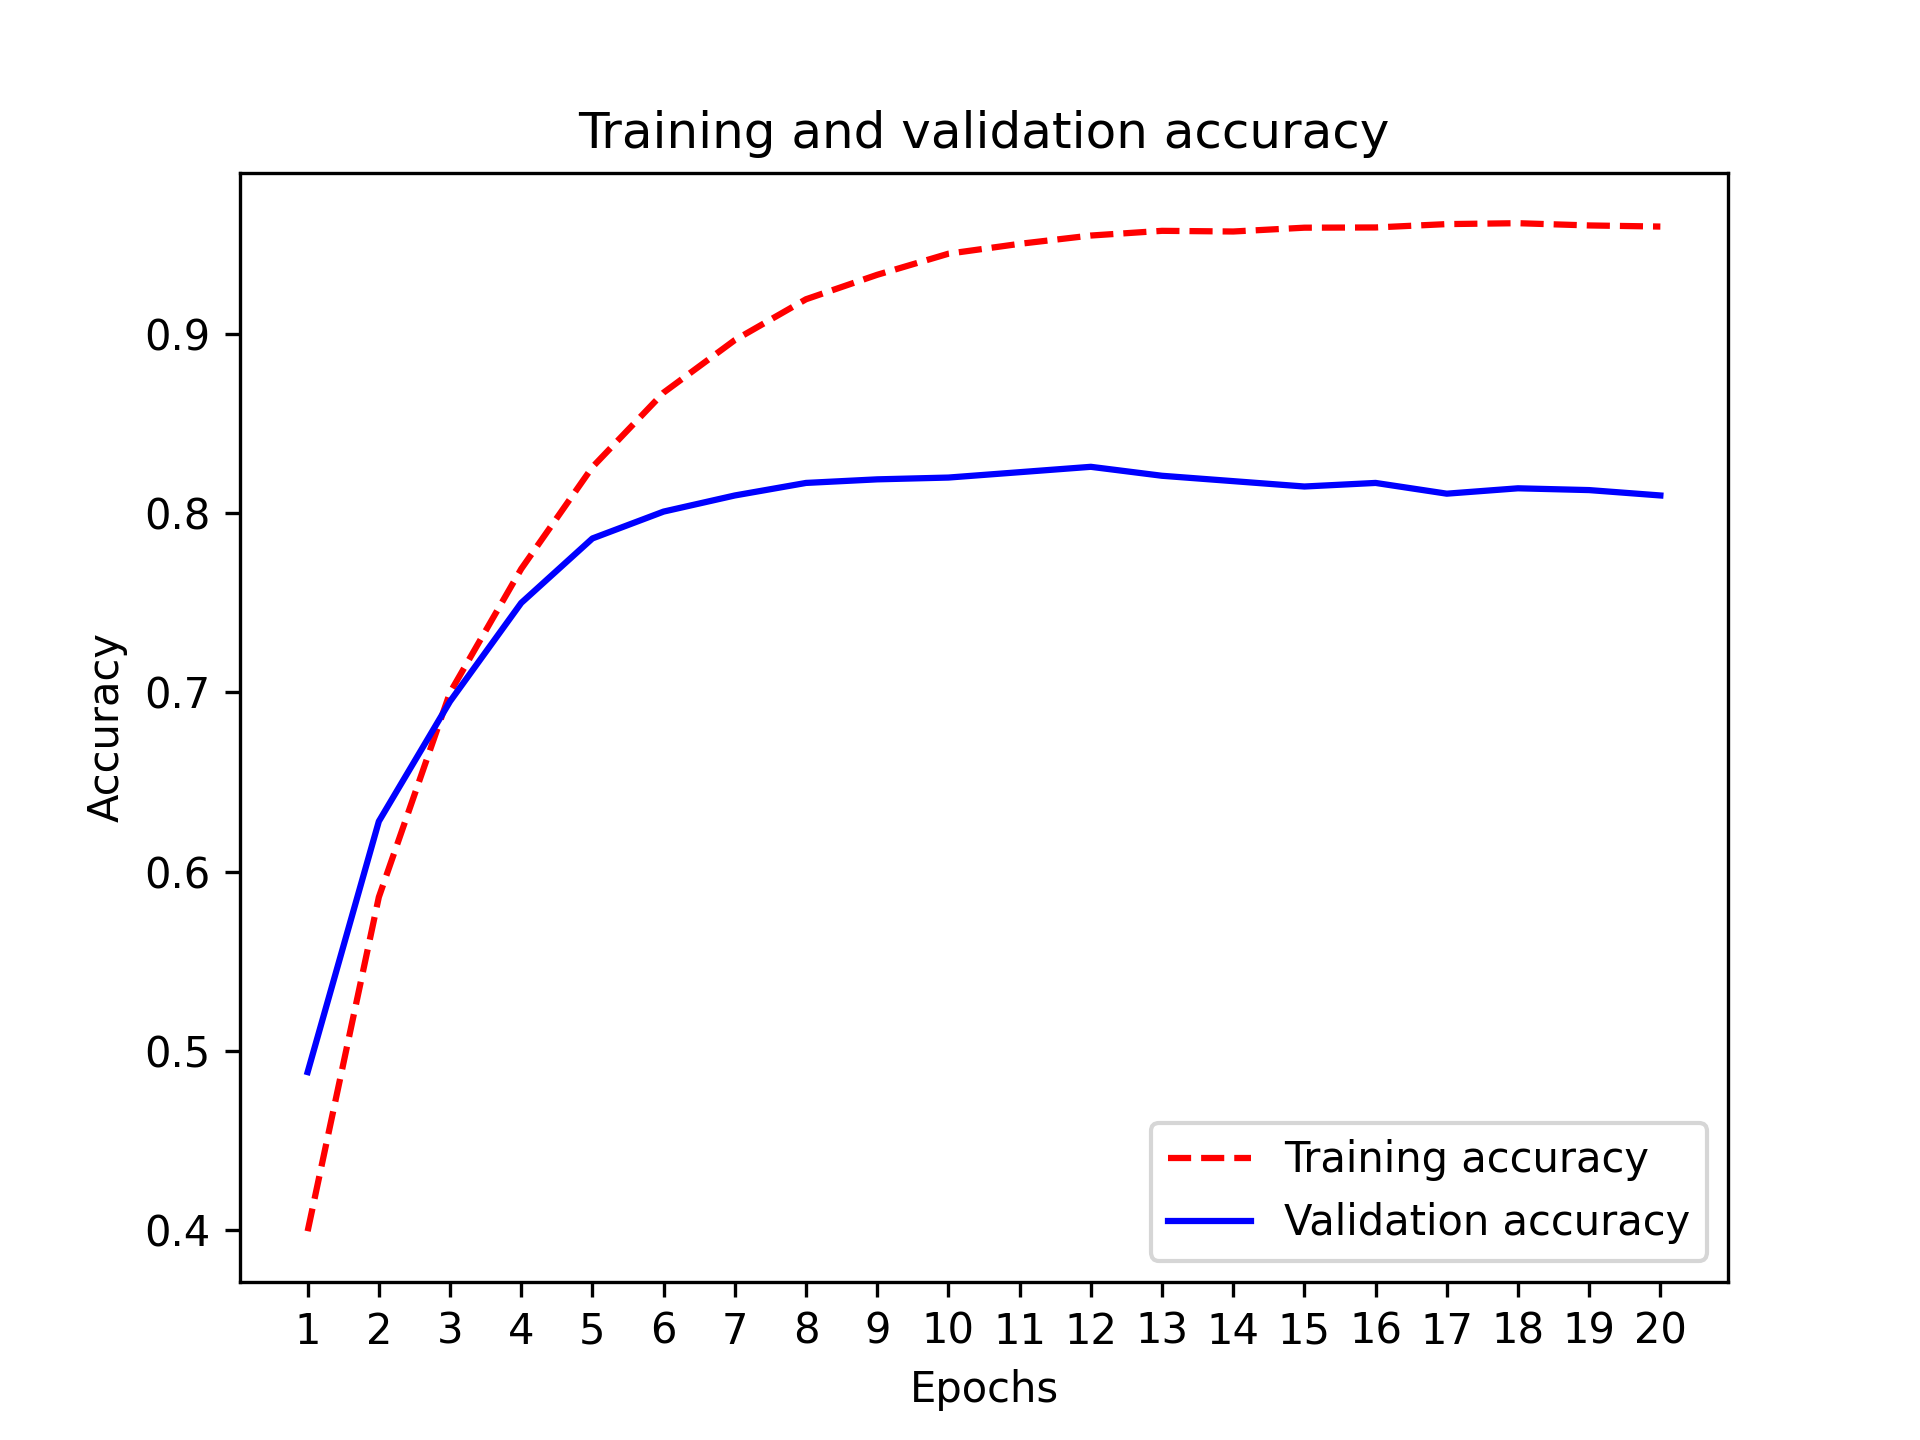
\includegraphics[width=\textwidth,height=0.7\textheight,keepaspectratio]{../../images/ch04/reuters_accuracy_plot.b74dee12.png}
            \caption{Training và Validation Accuracy}
        \end{figure}
    \end{columns}
\end{frame}

\begin{frame}{Nhưng 80\% đã là con số thực? (Top-3 Accuracy)}
    \begin{columns}
        \column{0.5\textwidth}
        \begin{itemize}
            \item Trong tin tức, một bài báo có thể liên quan tới cả 2, 3 chủ đề đan xen. Nếu dự đoán đúng của mô hình là lựa chọn xếp thứ hai hoặc thứ ba thì đó vẫn là thông tin có giá trị.
            \item \textbf{Top-3 Accuracy:} Đo lường xem tỷ lệ nhãn thật (Ground-truth) có nằm trong 3 phán đoán có xác suất cao nhất hay không.
            \item Chỉ số Top-3 này có thể lên tới >90\%.
        \end{itemize}
        
        \column{0.5\textwidth}
        \begin{figure}
            \centering
            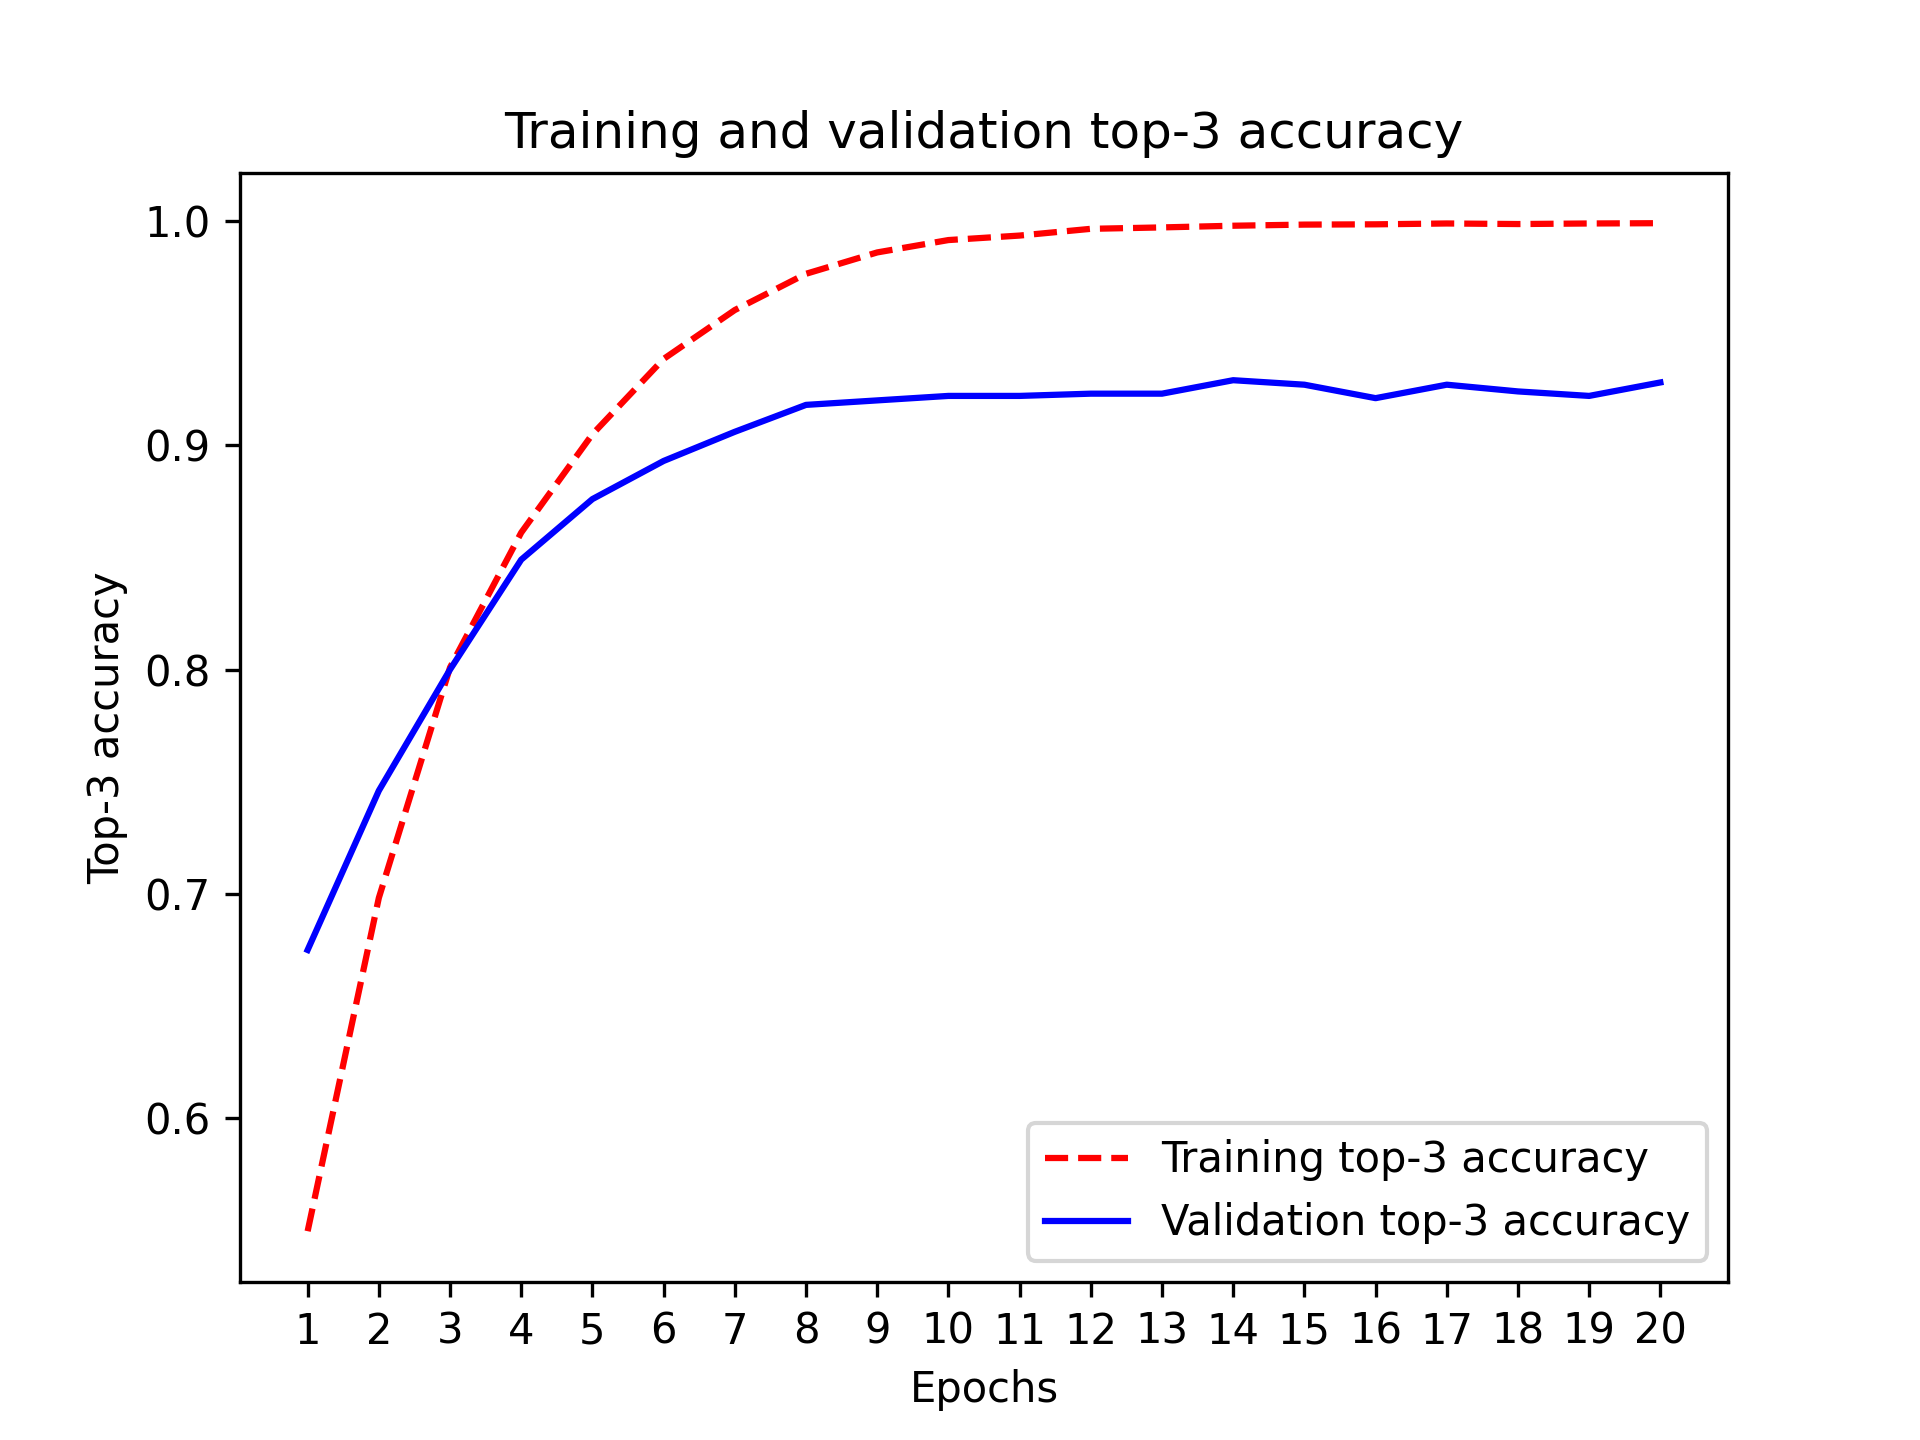
\includegraphics[width=\textwidth,height=0.7\textheight,keepaspectratio]{../../images/ch04/reuters_top_3_accuracy_plot.a9e13ec0.png}
            \caption{Chỉ số Top-3 Accuracy}
        \end{figure}
    \end{columns}
\end{frame}

\section{4. Hồi quy Vô hướng (Boston Housing)}

\begin{frame}{Bài toán Dự đoán Giá nhà Boston (Scalar Regression)}
    \begin{itemize}
        \item \textbf{Mục tiêu:} Dự đoán giá nhà trung bình tại vùng ngoại ô Boston (thập niên 1970) dựa trên 13 đặc trưng (tỷ lệ tội phạm, thuế, số phòng...).
        \item \textbf{Khác biệt lớn nhất:} Đầu ra không phải là "xác suất" hay "lớp", mà là \textbf{một con số vô hướng liên tục} (Ví dụ: Dự đoán căn nhà giá 25.000 Đô la). 
        \item Tập dữ liệu này cực kỳ nhỏ, chỉ có 506 mẫu. Trong đó 404 mẫu huấn luyện và 102 mẫu kiểm tra.
    \end{itemize}
\end{frame}

\begin{frame}[fragile]{Tiền xử lý: Chuẩn hóa Dữ liệu (Feature Scaling)}
    Các đặc trưng dữ liệu (tội phạm, diện tích, tuổi nhà) có thang đo hoàn toàn khác nhau. Đưa trực tiếp vào mạng nơ-ron sẽ gây khó khăn cho hội tụ trọng số. Ta phải chuẩn hóa \textbf{(Normalization)}: Trừ đi trung bình và chia cho độ lệch chuẩn.
\begin{lstlisting}[language=Python]
mean = train_data.mean(axis=0)
train_data -= mean
std = train_data.std(axis=0)
train_data /= std

# Can phai chuan hoa tap test theo trung binh cua tap train
test_data -= mean
test_data /= std
\end{lstlisting}
\end{frame}

\begin{frame}[fragile]{Xây dựng Mạng lưới Hồi quy}
    Do dữ liệu ít, ta chỉ dùng mạng nơ-ron nhỏ (2 lớp ẩn, 64 units) để tránh Overfitting mạnh.
\begin{lstlisting}[language=Python]
def build_model():
    model = keras.Sequential([
        layers.Dense(64, activation="relu"),
        layers.Dense(64, activation="relu"),
        layers.Dense(1) # Linear Layer - KHONG co ham kich hoat
    ])
    # Loss MSE chuyen de tinh loi hoi quy
    # Metric MAE de con nguoi de doc (Mean Absolute Error)
    model.compile(optimizer="rmsprop", loss="mse", metrics=["mae"])
    return model
\end{lstlisting}
\end{frame}

\begin{frame}{Đặc thù Dữ liệu Nhỏ \& K-Fold Cross-Validation}
    \begin{columns}
        \column{0.5\textwidth}
        \begin{itemize}
            \item Tập dữ liệu chỉ có 404 mẫu huấn luyện. Việc tách 100 mẫu ngẫu nhiên ra làm tập Validation sẽ gây ra phương sai sai số rất lớn, phụ thuộc vào "bốc trúng" dữ liệu dễ hay khó.
            \item \textbf{Giải pháp: K-Fold Cross Validation} (Thẩm định chéo K-lần).
            \item Tách tập train làm K phần bằng nhau ($K=4$). Mỗi lần dùng 1 phần để validation, 3 phần kia để train. Kết quả là trung bình của K vòng chạy.
        \end{itemize}
        
        \column{0.5\textwidth}
        \begin{figure}
            \centering
            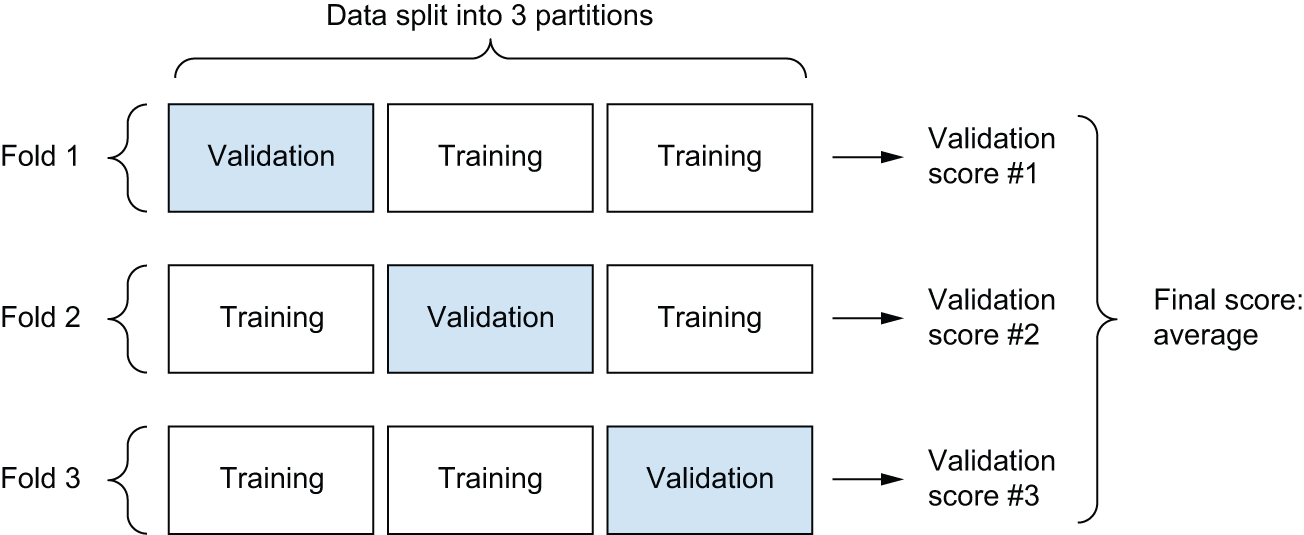
\includegraphics[width=\textwidth,height=0.7\textheight,keepaspectratio]{../../images/ch04/3-fold-cross-validation.40bb5356.png}
            \caption{Mô phỏng K-Fold Cross-Validation (K=3)}
        \end{figure}
    \end{columns}
\end{frame}

\begin{frame}[fragile]{Cài đặt K-Fold Validation}
\begin{lstlisting}[language=Python]
k = 4
num_val_samples = len(train_data) // k
all_mae_histories = []

for i in range(k):
    val_data = train_data[i * num_val_samples: (i + 1) * num_val_samples]
    val_targets = train_targets[i * num_val_samples: (i + 1) * num_val_samples]
    # Ghep du lieu cac fold khac de lam tap huan luyen
    partial_train_data = np.concatenate([
        train_data[:i * num_val_samples],
        train_data[(i + 1) * num_val_samples:]], axis=0)
    ...
    # model = build_model()
    # model.fit(...)
\end{lstlisting}
\end{frame}

\begin{frame}{Đánh giá Hiệu suất Hồi quy (MAE Plot)}
    \begin{columns}
        \column{0.5\textwidth}
        \begin{itemize}
            \item Khác với Accuracy (càng cao càng tốt), MAE (Mean Absolute Error) biểu thị cho sai số trung bình (càng thấp càng tốt). MAE = 0.5 tương đương sai lệch 500 Đô la.
            \item Trực quan hóa giá trị trung bình MAE qua K-folds trên 500 epochs.
            \item Đường đồ thị có độ rung (nhiễu) cao ở những epochs đầu.
        \end{itemize}
        
        \column{0.5\textwidth}
        \begin{figure}
            \centering
            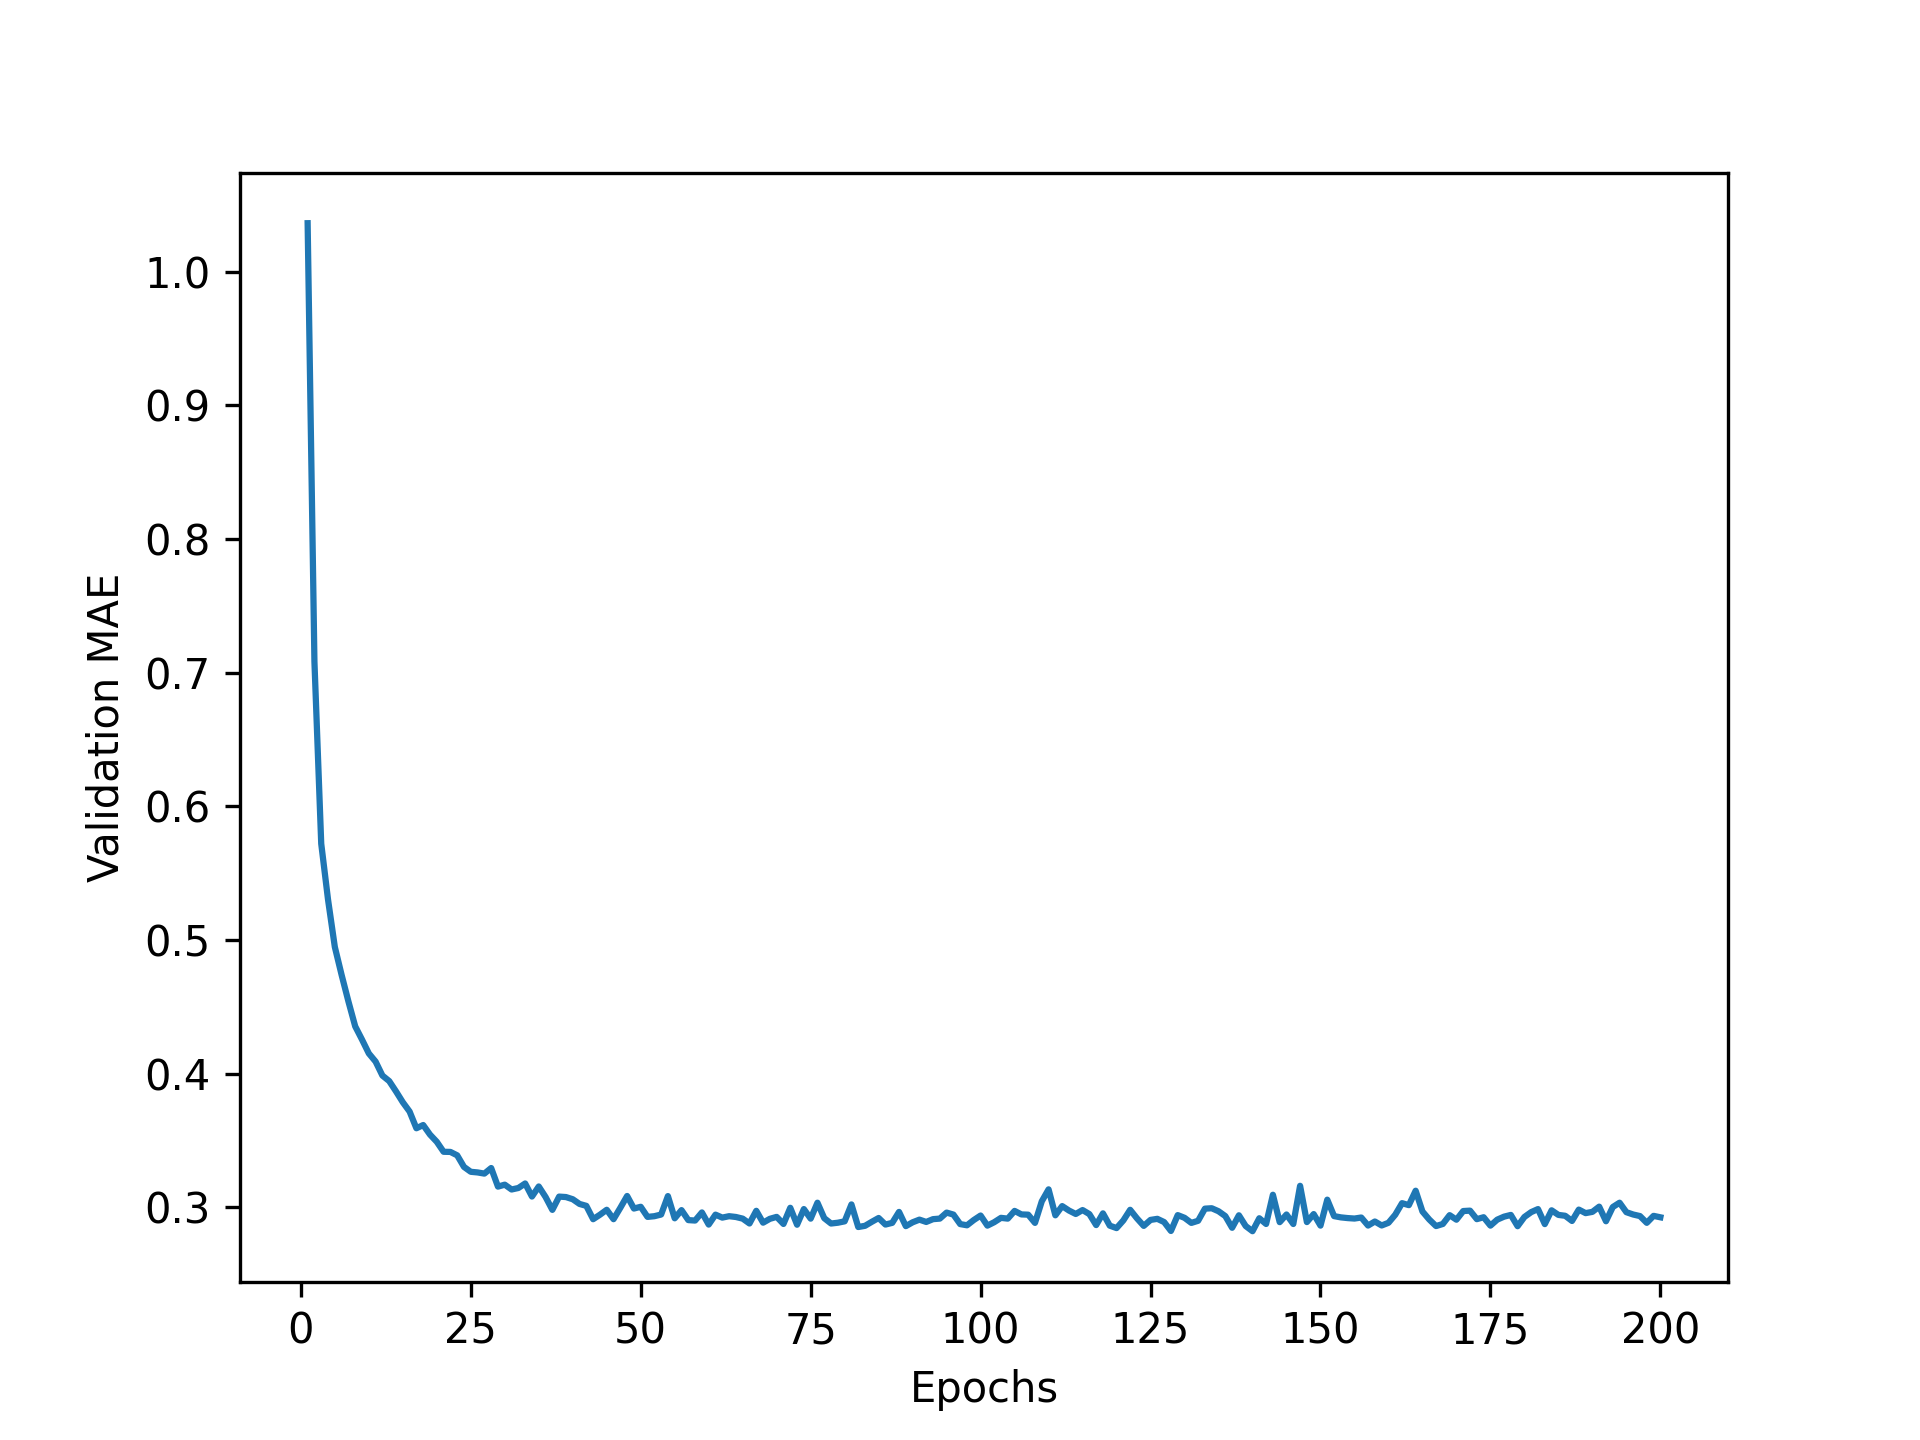
\includegraphics[width=\textwidth,height=0.7\textheight,keepaspectratio]{../../images/ch04/california_housing_validation_mae_plot.af306c57.png}
            \caption{Validation MAE qua 500 epochs}
        \end{figure}
    \end{columns}
\end{frame}

\begin{frame}{Phân tích Chuyên sâu (MAE Zoomed Plot)}
    \begin{columns}
        \column{0.5\textwidth}
        \begin{itemize}
            \item Bỏ qua 10 epochs đầu tiên vì sai số quá lớn làm lệch thang đo biểu đồ.
            \item Vẽ đường làm trơn (Exponential Moving Average) để quan sát rõ hơn xu hướng học.
            \item Đồ thị chạm đáy tối ưu ở khoảng 120-140 epochs, sau đó bắt đầu tăng vọt $\rightarrow$ \textbf{Overfitting} trên tập dữ liệu hồi quy.
        \end{itemize}
        
        \column{0.5\textwidth}
        \begin{figure}
            \centering
            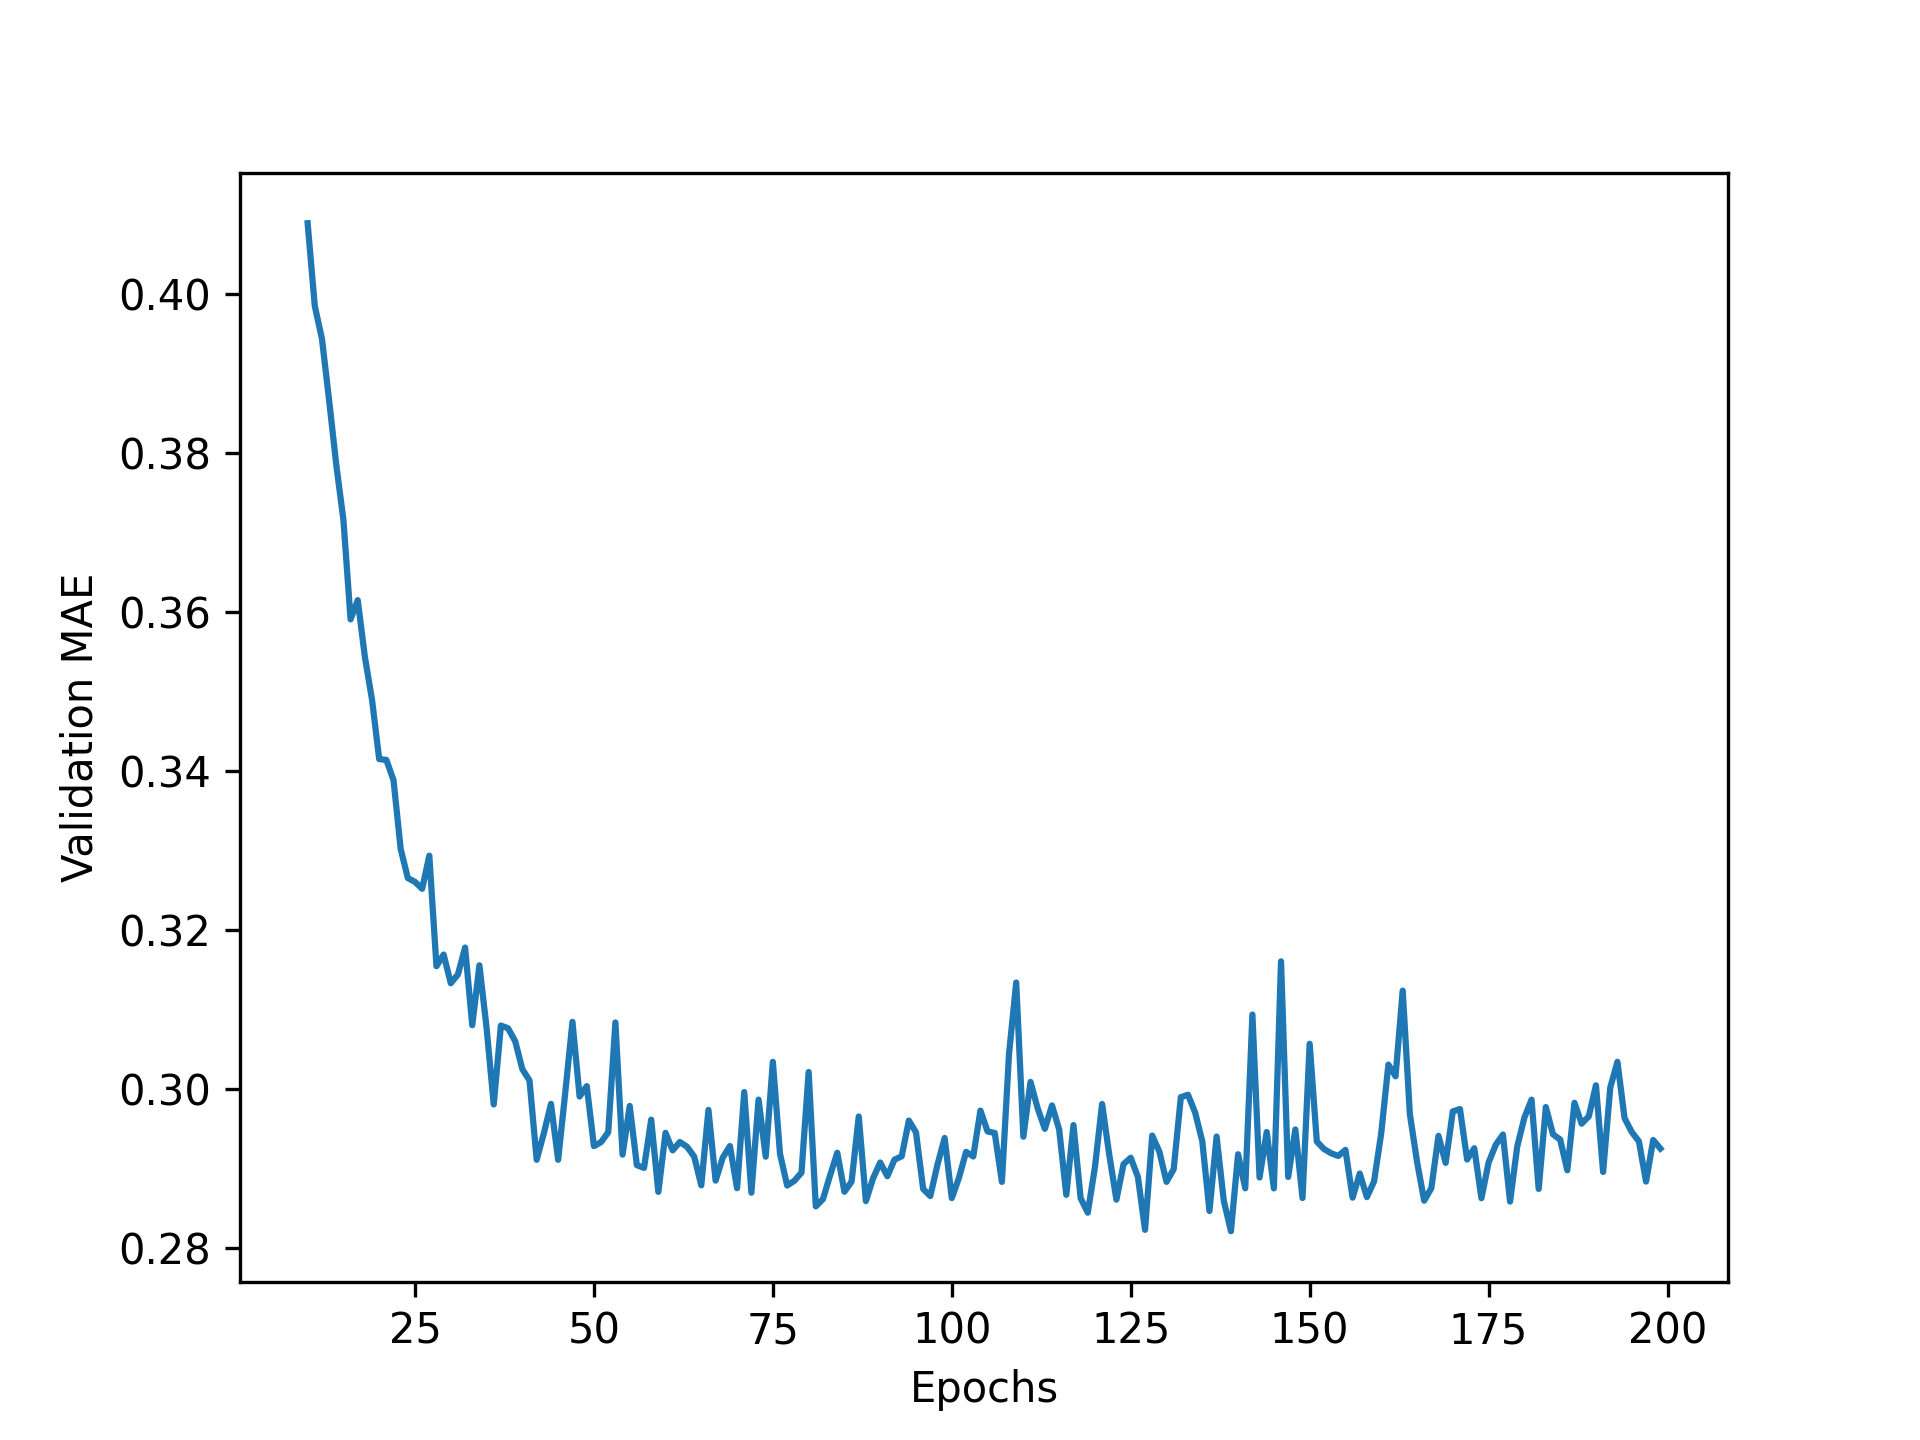
\includegraphics[width=\textwidth,height=0.7\textheight,keepaspectratio]{../../images/ch04/california_housing_validation_mae_plot_zoomed.928f390d.png}
            \caption{Đồ thị làm trơn (Zoomed)}
        \end{figure}
    \end{columns}
\end{frame}

\begin{frame}[fragile]{Huấn luyện chung cuộc và Dự đoán}
    Sau khi xác định được \texttt{epochs=130} là điểm tốt nhất, ta huấn luyện mô hình trên toàn bộ tập train và chạy test.
\begin{lstlisting}[language=Python]
model = build_model()
model.fit(train_data, train_targets, epochs=130, batch_size=16, verbose=0)

test_mse, test_mae = model.evaluate(test_data, test_targets)
print(test_mae) # Khoang 2.5 (Sai lech khoang $2,500)

predictions = model.predict(test_data)
print(predictions[0]) # Mang ket qua scalar
# VD: array([28.34494], dtype=float32) -> Can nha co gia 28,344$
\end{lstlisting}
\end{frame}

\section{Tổng kết}

\begin{frame}{Bảng tổng kết tra cứu nhanh}
    Khi bắt đầu dự án Học máy Vector (Bảng), hãy tuân theo quy tắc sau đối với Lớp Output:
    \begin{table}[h]
        \centering
        \begin{tabular}{@{}lllc@{}}
        \toprule
        \textbf{Bài toán} & \textbf{Kích hoạt Output} & \textbf{Hàm mất mát (Loss)} & \textbf{Metric} \\ \midrule
        Phân loại nhị phân & \texttt{sigmoid} (1 unit) & \texttt{binary\_crossentropy} & \texttt{accuracy} \\ 
        Phân loại đa lớp & \texttt{softmax} (N units) & \texttt{categorical\_crossentropy} & \texttt{accuracy} \\ 
        Hồi quy vô hướng & Tuyến tính (Linear) & \texttt{mse} (Mean Squared) & \texttt{mae} \\ \bottomrule
        \end{tabular}
    \end{table}
\end{frame}

\begin{frame}{Bài học rút ra từ Chương 4}
    \begin{itemize}
        \item \textbf{Tiền xử lý (Preprocessing):} Dữ liệu thô luôn phải được mã hóa dạng One-hot hoặc Chuẩn hóa (Normalization) các đặc trưng không cùng tỷ lệ trước khi đưa vào Mạng Nơ-ron.
        \item \textbf{Nút thắt cổ chai thông tin (Information Bottleneck):} Đối với các mạng đa lớp lớn (như Reuters 46 lớp), nếu chọn lớp ẩn quá nhỏ (vd: 16 units), thông tin sẽ bị đánh rơi vĩnh viễn.
        \item \textbf{Khắc tinh Overfitting:} Mạng nơ-ron LUÔN LUÔN bị quá khớp (overfit) sau một lượng thời gian nhất định. Cần theo dõi biểu đồ Loss trên Validation Set để biết thời điểm nên \textbf{Dừng sớm (Early Stopping)}.
        \item \textbf{Dữ liệu quá nhỏ (Small Data):} Rất dễ bị rung lắc mạnh khi tách Validation rời, hãy nghĩ đến \textbf{K-Fold Cross Validation}.
    \end{itemize}
\end{frame}

\end{document}
